% Options here are passed to the article class.
% Most common options: 10pt, 11pt, 12pt
\documentclass[10pt]{datasheet}

% Input encoding and typographical rules for English language
\usepackage[utf8]{inputenc}
\usepackage[english]{babel}
\usepackage[english]{isodate}

% tikz is used to draw images in this example, but you can
% also use \includegraphics{}.
\usepackage{graphicx}

% These define global texts that are used in headers and titles.
\title{DC01: 6 Bit Binary Decoder}
\author{Dzreams}
\tags{decoders, binary}
\date{October 2022}
\revision{Revision 1}

\begin{document}
\maketitle

\section{Features}

\begin{itemize}
\item{Constant time decoding. 14gt latency.}
\item{Slim profile. 4 blocks wide.}
\item{6gt throughput.}
\item{QC based logic.}
\end{itemize}

\section{Applications}

\begin{itemize}
\item{Decoding binary signals for use in external bulk systems}
\end{itemize}

\section{General Description}
The DC01 decoder takes six bits and outputs a pulse at one of 64 slices corresponding to the code.
% Switch to next column
\vfill\break

\begin{figure}[h]
    \centering
    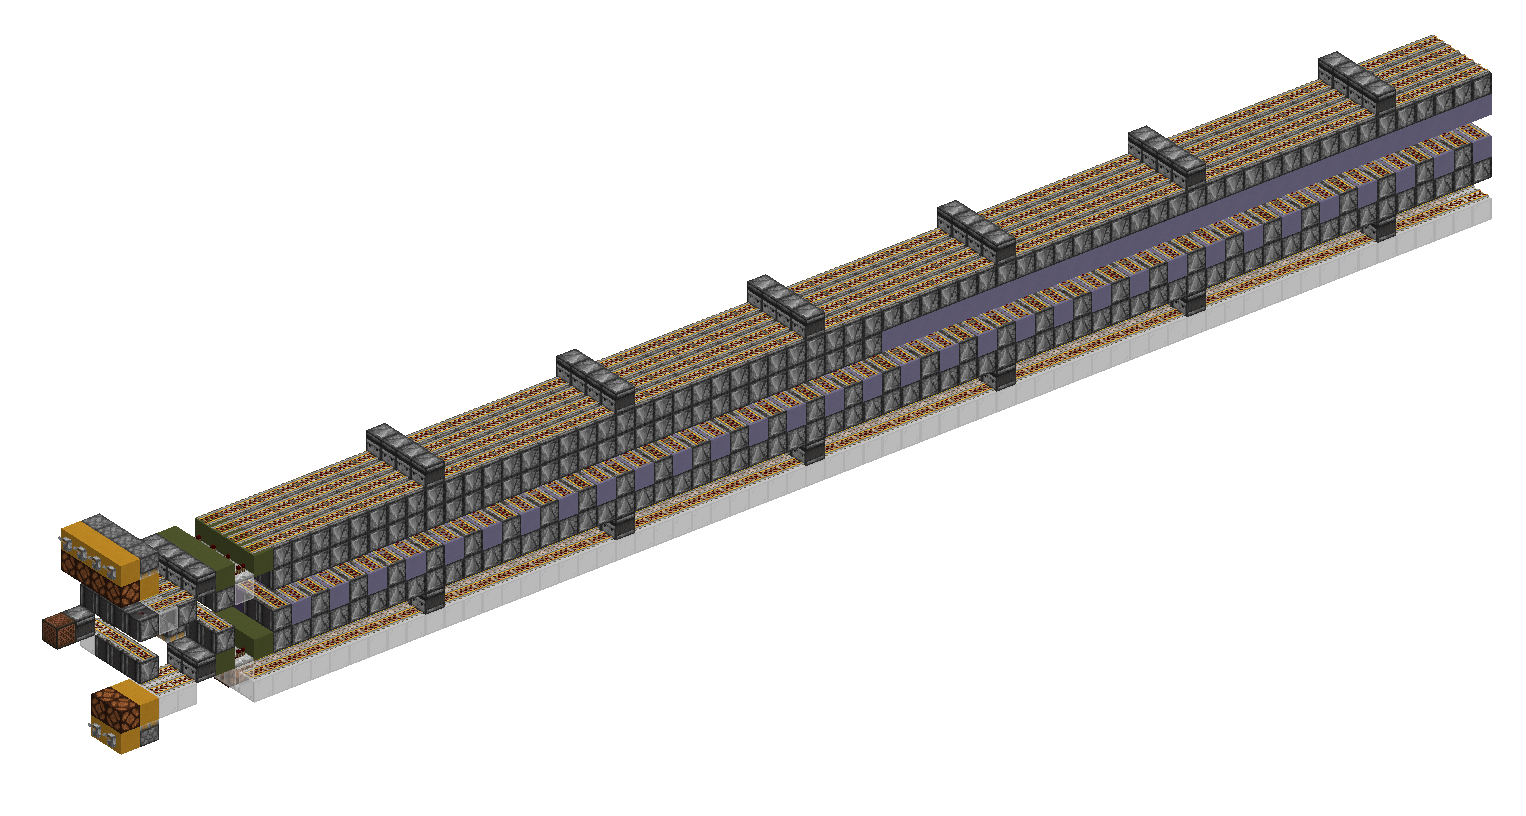
\includegraphics[width=0.45\textwidth]{6bit.png}
    \caption{\centering 6 Bit Binary Decoder}
\end{figure}

% For wide tables, a single column layout is better. It can be switched
% page-by-page.
\onecolumn

\section{Device Specifications}

\begin{table}[h]
    \caption{Inputs}
    \begin{tabularx}{\textwidth}{l | c | X}
        \thickhline
        \textbf{Name} & \textbf{Range} & \textbf{Description} \\
        \hline
        Bits 1-6 & 0-1 & Binary input \\
        \hline
        Execute & Pulse & Clock signal of device. \\
        \thickhline
\end{tabularx}
\end{table}

\begin{table}[h]
    \caption{Outputs}
    \begin{tabularx}{\textwidth}{l | c | X}
        \thickhline
        \textbf{Name} & \textbf{Range} & \textbf{Description} \\
        \hline
        Mapped signal & Pulse & Outputs to one of 64 slices corresponding to input code. \\
        \thickhline
\end{tabularx}
\end{table}

\begin{table}[h]
    \caption{Device Specifications}
    \begin{tabularx}{\textwidth}{l | c c c | c | X}
        \thickhline
        \textbf{Parameter} & \textbf{Min.} & \textbf{Typ.} & \textbf{Max.} &
        \textbf{Unit} & \textbf{Conditions} \\
        \hline
        Throughput  & 6 & 8 & - & gt & Normal Usage \\
        \hline
        Latency  & 14 & - & - & gt & Input to Output \\
        \hline
        Active Lag & +4.0 & 4.5 & +5.0 & ms & At Hopperspeed. Ryzen 5 3600, 2GB RAM. MC 1.18.1 with Lithium. \\
        \hline
        MC Version & 1.16 & 1.17.1 & - & MCV & Latest version at time of writing: 1.19.2\\
        \hline
        Dimensions & & 73 x 10 x 4 & & Blocks & \\
        \thickhline
\end{tabularx}
\end{table}

\newpage
\section{Testing Data}

\begin{table}[h]
\caption{Executed Tests}
\begin{tabularx}{\textwidth}{l | X}
    \thickhline
    \textbf{Test} & \textbf{Result} \\
    \hline
    Code test & Device was able to decode all possible codes successfully.\\
    \hline
    Throughput test & Device was able to decode at 6gt-8gt throughput.\\
    \thickhline
\end{tabularx}
\end{table}

\section{Download Information}
\begin{table}[h]
    \caption{Download Information}
    \begin{tabularx}{\textwidth}{l | l | l | X}
        \thickhline
        \textbf{Identifier} & \textbf{MC} & \textbf{File} & \textbf{Description} \\
        \hline
        DC01 & 1.17.1 & DC01\_6bit\_decoder.litematic & Litematic of decoder. \\
        \thickhline
    \end{tabularx}
\end{table}
\end{document}

